\chapter{Räumliches Lernen auf Graphen}
\label{raeumliches_lernen}

Das \emph{räumliche Lernen auf Graphen} basiert auf der direkten Überführung der Definition einer Faltung auf zweidimensionalen Bildern \bzw{} regulären Gittern über ein räumlich verschiebbares Fenster.
Ähnlich wie die Faltung in \glspl{CNN} wird dafür über eine Anordnung der Knoten mit festgelegter Schrittweite iteriert und für diese jeweils eine feste Menge an Nachbarsknoten bestimmt, die das Fenster \bzw{} das Receptive-Field eines jeden Knotens beschreiben~\cite{patchy}.
Aufgrund der gleichmäßigen räumlichen Anordnung der Pixel \bzw{} Knoten auf einem regulären Gitter ist die Definition einer Abtastfolge der Knoten und einer jeweiligen Nachbarschaftsbestimmung mit fester Größe und Ordnung recht trivial, wohingegen solche Definitionen im Kontext von willkürlichen Graphen aufgrund ihrer \ggf{} fehlenden räumlichen (oder zeitlichen) Anordnung nicht gleich ersichtlich erscheinen.

\citeauthor{patchy} definieren in ihrer Arbeit~\cite{patchy} einen solchen räumlichen Faltungsoperator auf Graphen, der im Folgenden vorgestellt und anschließend in den Kontext von Graphen im zweidimensionalen euklidischen Raum überführt wird.

\section{Grundlagen}
\label{raeumliche_grundlagen}

Für die Definition eines räumlichen Faltungsoperators auf Graphen werden spezielle Konstrukte der Graphentheorie benötigt, die im Folgenden vorgestellt werden.

\paragraph{Färbung von Knoten}
\label{faerbung_von_knoten}

Eine \emph{Knotenfärbung} $\gls{l}$ ist eine nicht zwingend injektive Funktion $\gls{l} \colon \gls{V} \to \gls{C}$ auf den Knoten eines Graphen \gls{G}, die jedem Knoten in \gls{V} eine \emph{Farbe} einer endlich abzählbaren Menge $\gls{C} \subseteq \gls{R}$ zuordnet~\cite{patchy}.
Mit Hilfe der Knotenfärbung lässt sich folglich eine Ordungsrelation $>_{\gls{l}}$ auf der Knotenmenge von \gls{G} definieren, wobei $\gls{v}_i >_{\gls{l}} \gls{v}_j$ genau dann, wenn $\gls{l}\left(\gls{v}_i\right) < \gls{l}\left(\gls{v}_j\right)$~\cite{patchy}.
Falls \gls{l} weiterhin injektiv ist, so spricht man von einer \emph{totalen Ordnung} und die Knoten $\gls{v} \in \gls{V}$ können insbesondere so permutiert werden, dass sie die Ordnung von $>_{\gls{l}}$ respektieren~\cite{patchy}.

Beispiele für eine Knotenfärbung sind Metriken, die die Wichtigkeit der einzelnen Knoten beschreiben.
Eine naive Metrik dafür ist \zB{} der Knotengrad \gls{degree} \bzw{} \gls{d}, der die \emph{Zentralität} der Knoten beschreibt~\cite{patchy}.
Komplexere Metriken für die Zentralität der Knoten sind unter anderem die Nähe, die Betweenness-Zentralität sowie die Eigenvektorzentralität~\cite{patchy, centrality}.
Letztere ist eng mit dem \emph{PageRank}-Algorithmus von Google verwandt ist~\cite{centrality}.
Die \emph{Nähe} (\engl{} \emph{Closeness})
\begin{equation*}
  c\left(\gls{v}\right) \coloneqq \frac{1}{\sum_{\gls{v}_i \in \gls{V}, \gls{v} \neq \gls{v}_i} \gls{s}\left(\gls{v}, \gls{v}_i\right)}
\end{equation*}
ist ein Maß für die durchschnittliche Länge zwischen einem Knoten und allen weiteren Knoten in \gls{V}~\cite{centrality}.
Je \emph{näher} ein Knoten sich an der Knotenmenge befindet, als desto zentraler gilt er.
Die \emph{Betweeness-Zentralität} eines Knotens $\gls{v} \in \gls{V}$ ist über
\begin{equation*}
  c\left(\gls{v}\right) \coloneqq \sum_{\gls{v}_i \neq \gls{v} \neq \gls{v}_j} \frac{\kappa_{ij}\left(\gls{v}\right)}{\kappa_{ij}}
\end{equation*}
definiert, wobei $\kappa_{ij} \in \gls{N}$ die Anzahl an kürzesten Pfaden von $\gls{v}_i$ nach $\gls{v}_j$ angibt und $\kappa_{ij}\left(\gls{v}\right) \in \gls{N}$ die Anzahl dieser Pfade beschreibt, die durch \gls{v} führen~\cite{centrality}.
Nach der Methode der \emph{Eigenvektorzentralität} gilt ein Knoten als umso wichtiger, je wichtiger seine Nachbarknoten sind~\cite{centrality}.
Sie ist definiert über
\begin{equation*}
  c\left(\gls{v}\right) = \frac{1}{\gls{lambda}} \sum_{\gls{v}_i \in \gls{Neighbor}\left(\gls{v}\right)} c\left(\gls{v}_i\right),
\end{equation*}
wobei $\gls{lambda} \in \gls{R}$.
Mit der Darstellung der Eigenvektorzentralität $c \colon \gls{V} \to \gls{R+}$ als Vektor $\ve{c} \in \gls{R+}^N$ und \gls{G} als ungewichtete Adjazenzmatrix $\gls{A} \in {\left\{0,1\right\}}^{N \times N}$ kann die Bestimmung von \gls{lambda} \bzw{} \ve{c} als Eigenwertproblem $\gls{A}\ve{c} = \gls{lambda}\ve{c}$ aufgefasst werden.
Dann beschreibt der größte Eigenwert \gls{lambda} die Eigenvektorzentralität der Knoten über dessen Eigenvektor \ve{c}~\cite{centrality}.

\paragraph{Isomorphie und kanonische Ordnung}
\label{isomorphie_und_kanonische_ordnung}

Seien $\gls{G}_1 = \left(\gls{V}_1, \gls{E}_1\right)$ und $\gls{G}_2 = \left(\gls{V}_2, \gls{E}_2\right)$ zwei Graphen mit der gleichen Anzahl an Knoten, \dhe{} $\left|\gls{V}_1\right| = \left|\gls{V}_2\right|$.
Dann heißt eine bijektive Abbildung $p \colon \gls{V}_1 \to \gls{V}_2$ \emph{Isomorphismus} zwichen $\gls{G}_1$ und $\gls{G}_2$, falls $\left(\gls{v}_i, \gls{v}_j\right) \in \gls{E}_1$ \gdw{} $\left(p\left(\gls{v}_i\right), p\left(\gls{v}_j\right)\right) \in \gls{E}_2$~\cite{nauty}.
Zwei Graphen sind \emph{isomorph} zueinander, falls ein Isomorphismus zwischen ihnen existiert.
Die Komplexität zur Bestimmung der Isomorphie zweier Graphen liegt in NP, wobei nicht bekannt ist, ob sie in P enthalten oder NP-vollständig ist~\cite{patchy}.

Die Komposition mehrerer Isomorphismen ist ebenfalls ein Isomorphismus~\cite{nauty}.
Die Menge aller Isomorphismen (zuzüglich der identischen Abbildung, die die Knoten auf sich selber abbildet) heißt die \emph{Isomorphismenklasse} des Graphen~\cite{nauty}.

Eine \emph{kanonische Ordnung} eines Graphen $\gls{G} = \left(\gls{V}, \gls{E}\right)$ ist ein Graph $\gls{G}^{\prime} = \left(\gls{V}^{\prime}, \gls{E}^{\prime}\right)$ mit einer eindeutigen Ordnung seiner Knoten $\gls{V}^{\prime}$, der isomorph zu \gls{G} ist und seine gesamte Isomorphismenklasse repräsentiert~\cite{patchy}.
Zwei Graphen sind insbesondere genau dann zueinander isomorph, wenn ihre kanonischen Ordnungen übereinstimmen~\cite{nauty}.
Abbildung~\ref{fig:kanonische_ordnung} illustriert das Prinzip einer kanonischen Ordnung anhand zwei einfach gewählter zueinander isomorpher Graphen.
\begin{figure}[t]
\centering
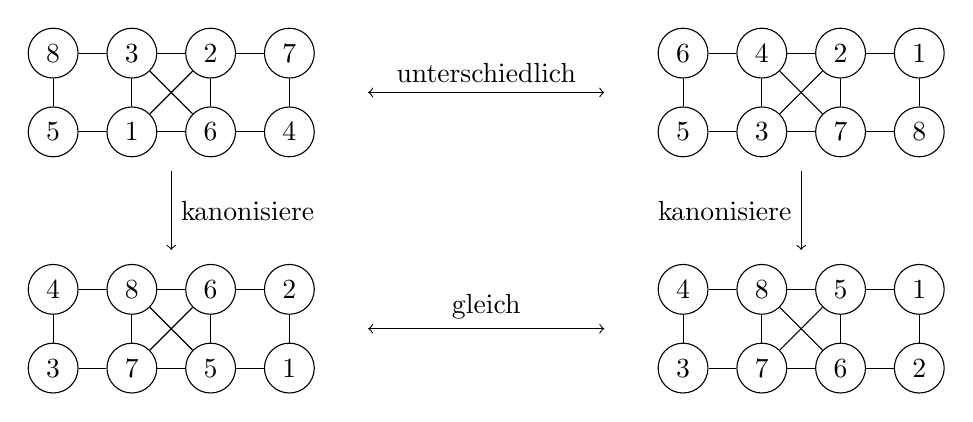
\begin{tikzpicture}
  \tikzstyle{node}=[circle,draw, minimum width=18pt, inner sep=0pt, fill=white]

  \node[node] (a1) at (0, 4) {$8$};
  \node[node] (a2) at (1, 4) {$3$};
  \node[node] (a3) at (2, 4) {$2$};
  \node[node] (a4) at (3, 4) {$7$};
  \node[node] (a5) at (0, 3) {$5$};
  \node[node] (a6) at (1, 3) {$1$};
  \node[node] (a7) at (2, 3) {$6$};
  \node[node] (a8) at (3, 3) {$4$};

  \path (a1) edge (a2);
  \path (a1) edge (a5);
  \path (a2) edge (a3);
  \path (a2) edge (a6);
  \path (a2) edge (a7);
  \path (a3) edge (a4);
  \path (a3) edge (a6);
  \path (a3) edge (a7);
  \path (a4) edge (a8);
  \path (a5) edge (a6);
  \path (a6) edge (a7);
  \path (a7) edge (a8);

  \node[node] (b1) at (0, 1) {$4$};
  \node[node] (b2) at (1, 1) {$8$};
  \node[node] (b3) at (2, 1) {$6$};
  \node[node] (b4) at (3, 1) {$2$};
  \node[node] (b5) at (0, 0) {$3$};
  \node[node] (b6) at (1, 0) {$7$};
  \node[node] (b7) at (2, 0) {$5$};
  \node[node] (b8) at (3, 0) {$1$};

  \path (b1) edge (b2);
  \path (b1) edge (b5);
  \path (b2) edge (b3);
  \path (b2) edge (b6);
  \path (b2) edge (b7);
  \path (b3) edge (b4);
  \path (b3) edge (b6);
  \path (b3) edge (b7);
  \path (b4) edge (b8);
  \path (b5) edge (b6);
  \path (b6) edge (b7);
  \path (b7) edge (b8);

  \node[node] (c1) at (8,  4) {$6$};
  \node[node] (c2) at (9,  4) {$4$};
  \node[node] (c3) at (10, 4) {$2$};
  \node[node] (c4) at (11, 4) {$1$};
  \node[node] (c5) at (8,  3) {$5$};
  \node[node] (c6) at (9,  3) {$3$};
  \node[node] (c7) at (10, 3) {$7$};
  \node[node] (c8) at (11, 3) {$8$};

  \path (c1) edge (c2);
  \path (c1) edge (c5);
  \path (c2) edge (c3);
  \path (c2) edge (c6);
  \path (c2) edge (c7);
  \path (c3) edge (c4);
  \path (c3) edge (c6);
  \path (c3) edge (c7);
  \path (c4) edge (c8);
  \path (c5) edge (c6);
  \path (c6) edge (c7);
  \path (c7) edge (c8);

  \node[node] (d1) at (8,  1) {$4$};
  \node[node] (d2) at (9,  1) {$8$};
  \node[node] (d3) at (10, 1) {$5$};
  \node[node] (d4) at (11, 1) {$1$};
  \node[node] (d5) at (8,  0) {$3$};
  \node[node] (d6) at (9,  0) {$7$};
  \node[node] (d7) at (10, 0) {$6$};
  \node[node] (d8) at (11, 0) {$2$};

  \path (d1) edge (d2);
  \path (d1) edge (d5);
  \path (d2) edge (d3);
  \path (d2) edge (d6);
  \path (d2) edge (d7);
  \path (d3) edge (d4);
  \path (d3) edge (d6);
  \path (d3) edge (d7);
  \path (d4) edge (d8);
  \path (d5) edge (d6);
  \path (d6) edge (d7);
  \path (d7) edge (d8);

  \draw[<->] (4,   3.5) -- node[above] {unterschiedlich} (7,   3.5);
  \draw[<->] (4,   0.5) -- node[above] {gleich}          (7,   0.5);
  \draw[->]  (1.5, 2.5) -- node[right] {kanonisiere}     (1.5, 1.5);
  \draw[->]  (9.5, 2.5) -- node[left]  {kanonisiere}     (9.5, 1.5);

\end{tikzpicture}
\caption[Kanoninsche Ordnung]{Illustration zweier isomorpher Graphen (oben), die jedoch nicht identisch sind (\zB{} sind die Knoten $1$ und $5$ im linken Graphen adjazent, aber nicht im rechten).
Der Prozess der Kanonisierung sorgt dafür, dass zwei isomorphe Graphen auch identisch sind (unten).
Die Kanten der Graphen verweisen jeweils auf die gleichen Indizes, auch wenn sich die Darstellung \bzw{} Position der Knoten unterscheidet.}
\label{fig:kanonische_ordnung}
\end{figure}


Ein Isomorphismus \bzw{} eine kanonische Ordnung kann ebenfalls eine Knotenfärbung \gls{l} berücksichtigen, indem Knoten durch einen Isomorphismus nur auf Knoten der gleichen Farbe abgebildet werden dürfen~\cite{nauty}.
Das reduziert die Menge der verfügbaren Isomorphismenklassen und insbesondere die Komplexität ihrer Berechnung.
Zur Berechnung der Isomorphismenklassen und der kanonischen Ordnung, auch unter Berücksichtigung einer Knotenfärbung, zeichnet sich das Programm \texttt{nauty} aufgrund dessen bemerkenswerter Berechnungslaufzeit aus (\vgl{}~\cite{nauty}).

\section{Spektraler Faltungsoperator}
\label{spektraler_faltungsoperator}

Sei $\ve{f} \in \gls{R}^N$ ein Signal auf den Knoten eines Graphen \gls{G}, welches abhängig von der Struktur des Graphen weiter verarbeitet werden soll.
Es ist jedoch nicht selbstverständlich, wie recht einfache, dennoch fundamentale Signalverarbeitungsprozesse wie Translation oder Filterung und die daraus entstehende Faltung in der Domäne des Graphen definiert werden können~\cite{Shuman}.
So kann \zB{} ein analoges Signal $f\left(t\right)$ mittels $f\left(t-3\right)$ um $3$ nach rechts verschoben werden.
Es ist hingegen völlig unklar was es bedeutet, ein Graphsignal auf den Knoten um $3$ nach rechts zu bewegen (\vgl{}~\cite{Shuman}).
Die spektrale Graphentheorie bietet uns dafür einen geeigneten Weg, in dem Eingabesignale in das Spektrum des Graphen zerlegt \bzw{} abgebildet, modifiziert und wieder retransformiert werden können.

\subsection{Graph-Fourier-Transformation}
\label{graph_fourier_transformation}

Das Spektrum eines Graphen \gls{G} bilden die Eigenwerte ${\left\{\gls{lambda}_i\right\}}_{i=1}^N$ der Laplace-Matrix \gls{Lboth} von \gls{G}.
Diese werden deshalb auch oft als die \emph{Frequenzen} von \gls{G} betitelt.
In der spektralen Domäne können wir ein Eingabeignal \ve{f} über \gls{G} dann analog wie ein zeitdiskretes Abtastsignal in der Fourier-Domäne behandeln.

\paragraph{Klassische Fourier-Transformation}
\label{klassische_fourier_transformation}

Die Fourier-Transformation $\hat f$ einer Funktion $f\left(t\right)$ ist definiert als~\cite{Shuman}
\begin{equation*}
  \hat f\left(\omega\right) \coloneqq \left\langle f, e^{2\pi i\omega t} \right\rangle = \int_{\gls{R}} f\left(t\right)e^{-2\pi i\omega t}\,\mathrm{d}t.
\end{equation*}
Die komplexen Exponentiale $e^{2\pi i\omega t}$ beschreiben dabei die Eigenfunktionen des eindimensionalen Laplace-Beltrami Operators~\cite{Shuman}
\begin{equation}
  - \nabla^2 e^{2\pi i\omega t} = - \frac{\partial^2}{\partial t^2} e^{2\pi i \omega t} = {\left(2\pi \omega\right)}^2 e^{2\pi i\omega t}.
  \label{eq:laplace_eigenfunktionen}
\end{equation}
$\hat f$ kann damit als die Ausdehnung von $f$ in Bezug auf die Eigenfunktionen des Laplace-Beltrami Operators $\nabla^2$ verstanden werden~\cite{Hammond}.
\\\\
Analog lässt sich die \emph{Graph-Fourier-Transformation} einer Funktion $f \colon \gls{V} \to \gls{R}$ \bzw{} $\ve{f} \in \gls{R}^N$ auf den Knoten eines Graphen \gls{G} als Ausdehnung von $f$ in Bezug auf die Eigenvektoren ${\left\{\gls{eiv}_i\right\}}_{i=1}^N$ der Laplace-Matrix \gls{Lboth} definieren~\cite{Shuman}:
\begin{equation}
  \hat f\left(\gls{lambda}_i\right) \coloneqq \left\langle \ve{f}, \gls{eiv}_i \right\rangle\, \text{\bzw{} } \ve{\hat f} \coloneqq \gls{Eiv}^{\top}\ve{f}.
  \label{eq:graph_fourier_transformation}
\end{equation}
Die inverse Graph-Fourier-Transformation ergibt sich dann als~\cite{Shuman}
\begin{equation}
  f\left(\gls{v}_i\right) = \sum_{j=1}^N \hat f\left(\gls{lambda}_j\right) {\left(\gls{eiv}_j\right)}_i\,\text{\bzw{} }\ve{f} = \gls{Eiv}\ve{\hat f}.
  \label{eq:inverse_graph_fourier_transformation}
\end{equation}

In der klassischen Fourier-Analyse sind für die Eigenwerte ${\left\{{\left(2\pi \omega\right)}^2\right\}}_{\omega \in \gls{R}}$ in~\eqref{eq:laplace_eigenfunktionen} nahe bei Null die korrespondieren Eigenfunktionen kleine, weich schwingende Funktionen, wohingegen für größere Eigenwerte \bzw{} Frequenzen die Eigenfunktionen sehr schnell und zügig anfangen zu oszillieren.
Bei der Graph-Fourier-Transformation ist dies ähnlich.
So ist für \gls{L} der erste Eigenvektor $\gls{eiv}_1 = \frac{1}{\sqrt{N}}{\left[1, \ldots, 1\right]}^{\top}$ zum Eigenwert $\gls{lambda}_1 = 0$ konstant und an jedem Knoten gleich.
Generell zeigt sich, dass die Eigenvektoren geringer Frequenzen nur geringfügig im Graph variieren, wohingegen Eigenvektoren größerer Eigenwerte immer unähnlicher werden (\vgl{}~\cite{Shuman}).
\\\\
Die Graph-Fourier-Transformation~\eqref{eq:graph_fourier_transformation} und ihre Inverse~\eqref{eq:inverse_graph_fourier_transformation} bieten uns eine Möglichkeit ein Signal in zwei unterschiedlichen Domänen zu repräsentieren, nämlich der Knotendomäne, \dhe{} das unveränderte Signal auf der Knotenmenge $f\left(\gls{v}_i\right)$, und der spektralen Domäne, \dhe{} das transformierte Signal in das Spektrum des Graphen $\hat f\left(\gls{lambda}_i\right)$.
Diese Transformation erlaubt uns die Formulierung fundamentaler Signalverarbeitungsoperationen.

\subsection{Spektrale Filterung}
\label{spektrale_filterung}

In der Signalverarbeitung versteht man unter der Frequenzfilterung die Transformation eines Eingabesignals in die Fourier-Domäne und der verstärkenden oder dämpfenden Veränderung der Amplituden der Frequenzkomponenten.
Formal betrachtet ergibt dies
\begin{equation}
  \hat f_{\mathrm{out}}\left(\omega\right) \coloneqq \hat f_{\mathrm{in}}\left(\omega\right)\hat g\left(\omega\right)
  \label{eq:fourier_filtering}
\end{equation}
mit dem Filter $\hat g \colon \gls{R} \to \gls{R}$.
\citeauthor{Shuman} zeigen, dass die Filterung in der Fourier-Domäne äquivalent zu einer Faltung in der Zeitdomäne ist, \dhe{}
\begin{equation}
  \left(f_{\mathrm{in}} \star g\right)\left(t\right) \coloneqq \int_{\gls{R}} f_{\mathrm{in}}\left(\tau\right)g\left(t - \tau\right)\, \mathrm{d}\tau = f_{\mathrm{out}}\left(t\right).
  \label{eq:fourier_faltung}
\end{equation}

Wir können die Filterung der Frequenzen in der Fourier-Domäne analog zu~\eqref{eq:fourier_filtering} für die spektrale Domäne auf Graphen über
\begin{equation*}
  \hat f_{\mathrm{out}}\left(\gls{lambda}_i\right) \coloneqq \hat f_{\mathrm{in}}\left(\gls{lambda}_i\right)\hat g\left(\lambda_i\right)\,\text{\bzw{} }\ve{\hat f}_{\mathrm{out}} \coloneqq \ve{\hat f}_{\mathrm{in}} \gls{hadamard} \ve{\hat g}
\end{equation*}
beschreiben, wobei \gls{hadamard} das elementweise Hadamard-Produkt ist~\cite{Shuman}.
$\ve{\hat g} \in \gls{R}^N$ ist damit ein \emph{nicht-parametrischer} Filter, \dhe{} ein Filter, dessen Werte für alle Frequenzen ${\left\{\gls{lambda}_i\right\}}_{i=1}^N$ frei wählbar sind~\cite{Defferrard}.
Daraus ergibt sich analog zu~\eqref{eq:fourier_faltung} der \emph{spektrale Faltungsoperator} auf Graphen in der Knotendomäne mit Hilfe der Graph-Fourier-Transformation~\eqref{eq:graph_fourier_transformation} und ihrer Inversen~\eqref{eq:inverse_graph_fourier_transformation} als~\cite{Shuman, Defferrard}
\begin{equation}
  \ve{f}_{\mathrm{in}} \star \ve{\hat g} \coloneqq \gls{Eiv}\left(\gls{Eiv}^{\top}\ve{f}_{\mathrm{in}} \gls{hadamard} \ve{\hat g}\right) = \ve{f}_{\mathrm{out}}.
  \label{eq:spektraler_faltungsoperator}
\end{equation}

\subsection{Polynomielle Approximation}
\label{polynomielle_approximation}

Es zeigt sich, dass die Benutzung des spektralen Faltungsoperators in~\eqref{eq:spektraler_faltungsoperator} im Kontext eines \glspl{CNN} auf Graphen mehrere Schwächen aufweist.
Es ist \zB{} leicht ersichtlich, dass die Auswertung von $\ve{f}_{\mathrm{in}} \star \ve{\hat g}$ extrem berechnungsintensiv ist.
So liegt die Laufzeit der Multiplikation mit der dichtbesetzten Eigenvektormatrix \gls{Eiv} in $\gls{O}\left(N^2\right)$, zudem muss \gls{Eiv} zuerst bestimmt werden — ein kostspieliger Aufwand für Graphen mit möglicherweise weit mehr als hundert Knoten~\cite{gcn}.
Desweiteren führt ein Filter $\ve{\hat g} \in \gls{R}^N$ der Größe $N$ zu einem Lernaufwand in $\gls{O}\left(N\right)$, \dhe{} der Dimensionalität der Eingabedaten~\cite{Defferrard}.
Ebenso kann $\ve{\hat g}$ so nicht für das Lernen auf unterschiedlich großen Graphen verwendet werden.

Um die oben genannten Schwächen zu umgehen kann $\hat g\left(\gls{lambda}_i\right)$ über ein Polynom\begin{equation}
  \hat g\left(\gls{lambda}_i\right) \approx \sum_{k=0}^K c_k\gls{lambda}_i^k \eqqcolon \hat g^{\prime}\left(\gls{lambda}\right)
  \label{eq:spektraler_filter_approximation}
\end{equation}
vom Grad $K$ mit Koeffizienten $c_0, \ldots, c_K \in \gls{R}$ approximiert werden~\cite{Hammond, Defferrard}.
Die Filtergröße von $\hat g^{\prime}$ sinkt somit auf einen konstanten Faktor $K$ mit Lernaufwand $\gls{O}\left(K\right)$, \dhe{} dem gleichen Aufwand klassischer zweidimensionaler \glspl{CNN}~\cite{Defferrard}.
$\ve{f}_{\mathrm{in}} \star \ve{\hat g}$ ergibt sich dann mittels~\eqref{eq:matrix_potenz},~\eqref{eq:spektraler_faltungsoperator} und~\eqref{eq:spektraler_filter_approximation} approximiert durch~\cite{Defferrard}
\begin{equation}
  \ve{f}_{\mathrm{in}} \star \ve{\hat g} \approx \sum_{k=0}^K c_k\gls{Eiv}\gls{Lambda}^k\gls{Eiv}^{\top}\ve{f}_{\mathrm{in}} = \sum_{k=0}^K c_k \gls{Lboth}^k \ve{f}_{\mathrm{in}}.
  \label{eq:spektraler_faltungsoperator_approximation}
\end{equation}
Insbesondere ist die spektrale Faltung damit nicht mehr abhängig von der Berechnung der Eigenwerte \bzw{} Eigenvektoren von \gls{Lboth}.
Mittels Kapitel~\ref{laplace_eigenschaften} kann $\ve{f}_{\mathrm{in}} \star \ve{\hat g}$ in der Knotendomäne nun als eine \emph{lokaliserte lineare Transformation} interpretiert werden.
So sammelt ein Summand $\gls{Lboth}^k\ve{f}_{\mathrm{in}}$ des spektralen Filters an einem Knoten \gls{v} genau die Signale von Knoten auf, die maximal $k$ Kanten von \gls{v} entfernt liegen~\cite{Hammond}.

\paragraph{Tschebyschow-Polynome}
\label{tschebyschow_polynome}

\todo{fettes todo}

\paragraph{Tensorimplementierung}
\label{tschebyschow_tensor}

\todo{fettes todo}

\section{Erweiterung auf Graphen im zweidimensionalen Raum}
\label{raeumliche_erweiterung}

\citeauthor{patchy} haben einen Algorithmus zur Generierung von Receptive-Fields über den Nachbarschaften eines Graphen vorgestellt, der effizient implementiert werden kann und über einer Reihe von Testdatensätzen konkurrenzfähige Resultate im Vergleich zu Methoden mittels \emph{Graphkernen} liefert (\vgl{}~\cite{patchy}).
Dabei hängt die Ordnung der Knotenauswahl und der Receptive-Fields stark von einer gewählten Zentralitätsmetrik ab, die auf einem allgemeinen Graphen $\gls{G} = \left(\gls{V}, \gls{E}\right)$ eine fehlende räumliche oder zeitliche Ordnung ersetzt.
Im Kontext von Graphen im zweidimensionalen euklidischen Raum $\gls{G} = \left(\gls{V}, \gls{E}, \gls{p}\right)$, bei denen Knoten eindeutige Positionen in der Ebene zugeordnet werden können und deren Kanten eine Länge und Richtung über $\gls{Adist} \in {\left[0, 1\right]}^{N \times N}$ sowie $\gls{Arad} \in {\left[0, 2\pi\right]}^{N \times N}$ besitzen, kann die Auswahl der Knoten in $\gls{V}_{\mathrm{out}}$ sowie die Normalisierung der Nachbarschaftsmenge $\gls{N}_{\gls{v}}$ eines Knotens $\gls{v} \in \gls{V}_{\mathrm{out}}$ diese jedoch folglich berücksichtigen.

Die Knotenauswahl kann folglich über die Anordnung der Knoten \bzgl{} ihrer \emph{Scanline} beschrieben werden, \dhe{} von oben nach unten und von links nach rechts.
Formal lässt sich dafür die Knotenfärbung $\gls{l}_{\mathrm{scanline}} \colon \gls{V} \to \gls{R}$ über
\begin{equation*}
  {\gls{l}_{\mathrm{scanline}}\left(\gls{v}\right)}^{-1} \coloneqq \frac{w_{\max}}{h_{\min}} {\hat p\left(\gls{v}\right)}_1 + {\hat p\left(\gls{v}\right)}_2
\end{equation*}
mit dem maximalen Breitenabstand $w_{\max} \coloneqq \max_{\gls{v}_i, \gls{v}_j \in \gls{V}} \left({\gls{p}\left(\gls{v}_i\right)}_2 - {\gls{p}\left(\gls{v}_j\right)}_2 \right)$ sowie dem minimalen Höhenabstand $h_{\min} \coloneqq \min_{\gls{v}_i, \gls{v}_j \in \gls{V},\, {\gls{p}\left(\gls{v}_i\right)}_1 \neq {\gls{p}\left(\gls{v}_j\right)}_1} \left({\gls{p}\left(\gls{v}_i\right)}_1 - {\gls{p}\left(\gls{v}_j\right)}_1 \right)$ und
\begin{equation*}
  \hat p\left(\gls{v}\right) \coloneqq {\left[{\gls{p}\left(\gls{v}\right)}_1 - y_{\min}, {\gls{p}\left(\gls{v}\right)}_2 - x_{\min}\right]}^{\top}
\end{equation*}
mit $y_{\min} \coloneqq \min \left({\gls{p}\left(\gls{v}_1\right)}_1, \ldots, {\gls{p}\left(\gls{v}_N\right)}_1\right)$ \bzw{} $x_{\min} \coloneqq \min \left({\gls{p}\left(\gls{v}_1\right)}_2, \ldots, {\gls{p}\left(\gls{v}_N\right)}_2\right)$ definieren, sodass Knoten einen höheren Farbwert erhalten, umso geringer ihre $y$-Koordinate ist und bei gleicher $y$-Koordinate ihre $x$-Koordinate die Farben weiter differenziert.
Dafür werden die Positionen $p$ mittels $\hat p$ in den positiven reellen transformiert und die $y$-Koordinate von $\hat p\left(\gls{v}\right)$ insofern gewichtet, dass für zwei unterschiedliche $y$-Koordinaten die Ordnung, die die Knotenfärbung generiert, nicht von der $x$-Koordinate abhängt.
Damit entspricht der Algorithmus~\ref{alg:knotenauswahl} mit der Knotenfärbung $\gls{l}_{\mathrm{scanline}}$ in etwa der Pixelauswahl einer klassischen Faltung auf regulären Gittern, mit dem Unterschied, dass die Knotenauswahl letztendlich eine eindimensionale geordnete Menge definiert.
Das ist aufgrund der möglichen Irregularitäten in den jeweiligen Knotenpositionen allerdings nicht zu vermeiden.
Folglich sind benachbarte Knoten in $\gls{V}_{\mathrm{out}}$ nicht zwangsläufig auch in der Ebene benachbart.
$\gls{l}_{\mathrm{scanline}}$ generiert jedoch eine Knotenfärbung, die für zwei strukturell gleiche Graphen eine ähnliche Ordnung generiert.


% Wir wollen, dass benachbarte Knoten im Receptive-Field ebenfalls benachbart im Bild sind

% beachtet keine Gewichte
% beatchtet keine Positionen
% im Kontext von Graphen im zweidimensionalen  euklidischen  Raum stehen uns diese aber zur Verfügung und sollten dementsprechen genutzt werden.
% Dafür wird das zuvor beschrieben Prinzip angepasst.

% Als Knotenauswahl wählen wir Stackline-Order?
% Für die Nachbarschaftsauswahl kombinieren wir die Auswahl und dessen Normalisierung zu einem Schritt.
% Spriale

% Für die Neighborhood Assembly eines Knotens wurde ein spezieller Algorithmus implementiert, der die nächsten Knoten um den Rootknoten ähnlich wie bei einer Spirale einsammelt.

% Dies wurde implementiert, da der eigentliche Gedanke, eine Convolution auf Basis des Grids, das SLIC erzeugt, nicht möglich ist. Es ist daher nicht möglich, da SLIC kein vollkommenes Grid erzeugt. Es werden teilweise Knoten hinzugefügt oder entfernt, wenn dies sinnvoll erscheint. Damit spuckt SLIC auch immer nur eine approximierte Anzahl an Segmenten aus, die gewünscht waren.

% Der Grid-Spiral-Algorithmus funktioniert wie folgt:

% Der Root Knoten ist immer an Index 0.
% Es wird der nächstgelegene Nachbar zum Rootknoten gesucht und der Neighborhood angehängt.
% Es wird wiederholt ein Nachbar y zum letzten hinzugefügten Knoten x gesucht, sodass $w(x, y)$ + $w(root, y)$ minimal.

\begin{algorithm}[t]
\centering
\begin{algorithmic}
  \REQUIRE{}
  \ENSURE{}
\end{algorithmic}
\caption[]{}
\label{alg:spirale}
\end{algorithm}

\section{Netzarchitektur}
\label{spektrale_netzarchitektur}

Die Architektur eines neuronalen Netzes auf Graphen mit spektralen Faltungen verhält sich durch die ähnliche Formulierung einer Faltungs- und einer Poo\-ling\-sch\-icht analog zu der Netzarchitektur klassischer \glspl{CNN}.
Dabei werden wie gewohnt mehrere Faltungsschichten mit stetig erhöhter Merkmalsausbreitung aneinander gereiht und an einigen Stellen über Poolingschichten getrennt, die die Anzahl der zu betrachtenden Knoten sukzessive reduzieren.
Im Anschluss darauf finden sich im Allgemeinen zwei bis drei vollverbundene Schichten, die die Merkmalsgröße dann schlussendlich auf die gewünschte Ausgabegröße reduzieren~\cite{Nielsen}.
Die mehrmalige Verkettung von Faltungsschichten sorgt dafür, dass auch bei einer relativ kleinen Faltung über die lokale Nachbarschaft eines jeden Knoten Merkmale weit entfernterer Knoten gewonnen werden können.

\glspl{CNN} auf Bildern erfordern dabei in einer analogen Netzarchitektur eine feste Eingabegröße.
Dafür werden die Bildermengen in der Regel insofern skaliert und zugeschnitten, dass diese alle die gleiche Bildgröße besitzen (\zB{} $224 \times 224$)~\cite{spp}.
Es erscheint jedoch schwierig, eine Menge von Graphen soweit anzupassen, dass diese alle die gleiche Anzahl an Knoten aufweisen.
So ist es zwar vorstellbar, zusätzliche \enquote{Fake}-Knoten zu jedem Graphen hinzufügen, damit diese alle eine feste Anzahl an Knoten aufweisen.
Neben dem erhöhtem Speicheraufwand ist dieser Ansatz jedoch insbesondere nicht geeignet für unbekannte Graphen, die in das Netz eingespeist werden.
So können diese \evtl{} eine größere Anzahl als die zuvor festgelegte Größe aufweisen.
Ebenso liefert uns der Prozess der Graphvergröberung eine stets unterschiedliche Repräsentation eines Graphen, die wohlmöglich bereits eine größere Menge an \enquote{Fake}-Knoten hinzufügt und dabei die festgelegte Knotengröße der Graphen überschreitet.
Es ist weiterhin schwierig, einen Graphen auf eine feste Größe zuzuschneiden.
So ist es insbesondere nicht ersichtlich, welche Knoten aus einem Graphen entfernt oder zusammengefasst werden können.

Die Architektur eines neuronalen Netzes auf Graphen erfordert folglich eine Struktur, die auf dynamischen Eingabegrößen operiert.
Dazu muss vorerst geklärt werden, warum ein klassisches \gls{CNN} auf Bildern eine feste Eingabegröße erfordert.
Eine einfache und elegante Lösung dazu bietet uns das \emph{Average-Pooling}, \dhe{} die Durchschnittsbildung eines Merkmals über allen Knoten.
Da die Anzahl der betrachteten Merkmale pro Knoten in jeder Schicht fest ist, liefert uns das Average-Pooling zwischen den Faltungs- und den vollverbundenen Schichten eines Netzes


Abbildung~\ref{fig:netzarchitektur_spectal} veranschaulicht die beschriebene typische spektrale Netzarchitektur.
\begin{figure}[t]
\centering
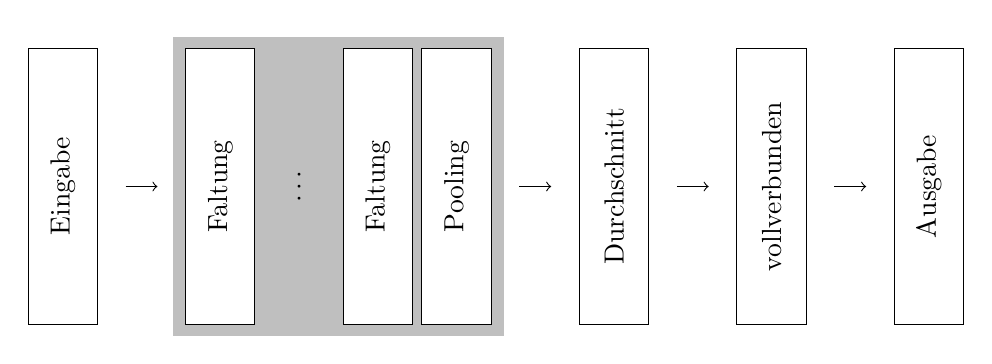
\begin{tikzpicture}[->, shorten >= 10pt, shorten <= 10pt]
  \tikzstyle{node}=[rectangle,draw, minimum width=100pt, minimum height=25pt, inner sep=0pt, fill=white, rotate=90]
  \tikzstyle{noborder}=[draw=none,fill=none]
  \tikzstyle{color1}=[fill=orange]

  \fill [lightgray] (1.4, -1.9) rectangle (5.6, 1.9) node {};

  \node[node] (0)  at (0, 0) {Eingabe};
  \node[node] (1)  at (2, 0) {Faltung};
  \node[node,noborder] (2)  at (3, 0) {$\ldots$};
  \node[node] (3)  at (4, 0) {Faltung};
  \node[node] (4)  at (5, 0) {Pooling};
  \node[node] (5)  at (7, 0) {Durchschnitt};
  \node[node] (6)  at (9, 0) {vollverbunden};
  \node[node] (7)  at (11, 0) {Ausgabe};

  \path (0) edge (1);
  \path (4) edge (5);
  \path (5) edge (6);
  \path (6) edge (7);
\end{tikzpicture}
\caption[Spektrale Netzarchitektur auf Graphen]{Typische spektrale Netzarchitektur auf Graphen bestehend aus beliebig vielen verketteten Faltungsschichten gefolgt von jeweils einer Poolingschicht.
Im Anschluss sorgt die Benutzung einer Durchschnittsschicht über den Knoten jedes Merkmals für die Verwendung von vollverbundenen Schichten hinzu zur Ausgabe.}
\label{fig:netzarchitektur_spectal}
\end{figure}

Alternative Architekturen, auch im Hinblick auf Ersetzungsmöglichkeiten des Average-Poolings, werden in Kapitel~\ref{ausblick} diskutiert.

